\begin{refsection}
% DK: I am not sure about the [old] title of this pattern. The bulk of the body of the pattern seems to be about the reuse. Maybe something like “Don’t Make what you can Use” might fit the spirit better. [fixed]

\paragraph{Context}
% DK: This seems like an explanation of the title, not a ``context'' in which a problem is observed.
In a peer production context, you are simultaneously ``making stuff'' and building on the work of others. 
\textbf{You don't have to do everything yourself!  The library of resources you can draw on is vast -- but it is useful only if you can make sense of it.}

%\vspace{.1cm}

\paragraph{Problem}
People are often very attached to their own projects and priorities and don't have a sense of how their initiatives can benefit from connection and relationship.  Many projects die because the cost of \patternnameext{\href{http://c2.com/cgi/wiki?ReinventingTheWheel}{Reinventing the Wheel}} [c2] is too high.

\paragraph{Solution} ``Steal like an artist,'' and make it possible for other people to build on your work too (Figure \ref{fountain}).  In the Peeragogy project, we have written very little new software, and have instead used off-the-shelf and hosted solutions suited to the task at hand (including: Drupal, Google+, Google Hangouts, Google Docs, Wordpress, pandoc, XeLaTeX, Authorea, and Github).  Early on we agreed to release our \emph{Peeragogy Handbook} under the terms of the Creative Commons Public Domain Dedication (CC0), the legal instrument that grants the greatest possible leeway to downstream users.\footnote{\url{https://creativecommons.org/publicdomain/zero/1.0/}}  This has allowed us and others to repurpose and improve its contents in other settings, including the current paper.  In short, follow the steps indicated by the keywords in the pattern's title:  \emph{Reduce} the panoply of interesting interrelated ideas and methods to a functional core (e.g.~writing a book).  \emph{Reuse} whatever resources are relevant to this aim, factoring in ``things I was going to have to do anyway'' from everyone involved.  \emph{Recycle} what you've created in new connections and relationships.

\begin{figure}
\begin{center}
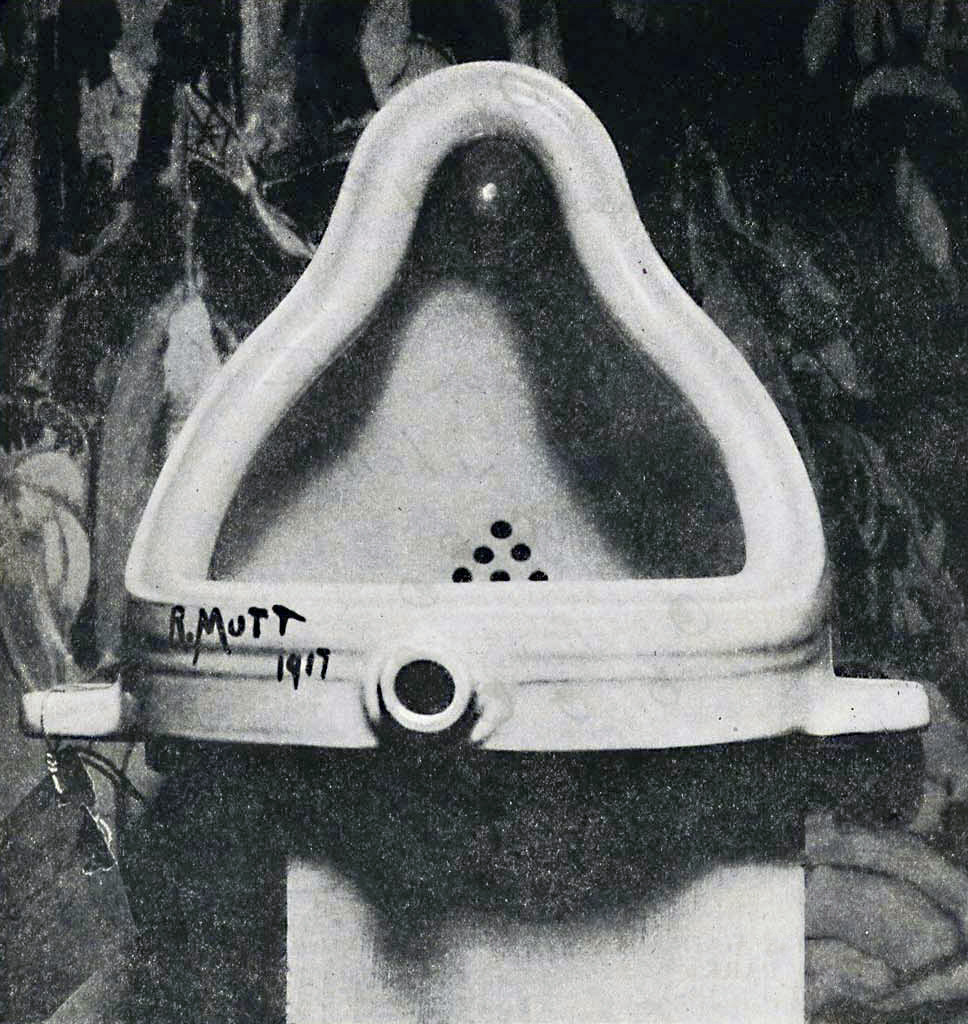
\includegraphics[width=.8\textwidth]{Duchamp_Fountaine.jpg}
\end{center}
\caption{A paradigmatic example of found-art. Caption reads: ``Fountain by R. Mutt, Photograph by Alfred Stieglitz, THE EXHIBIT REFUSED BY THE INDEPENDENTS''. Public domain, via the Wikimedia Commons.\label{fountain}}
%\vspace{-.cm}
\end{figure}

%\vspace{.2cm}

\paragraph{Rationale} 
Clearly we are not the first people to notice the problems with wheel-reinvention, including ``missing opportunities, repeating common mistakes, and working harder than we need to.''\footnote{\url{https://blog.wikimedia.org/2013/11/19/learning-patterns-new-way-share-important-lessons/}}  As a guest in one of our hangouts, Willow Brugh, of Geeks without Bounds and the MIT Media Lab, remarked that \emph{people often think that they need to build a community, and so fail to recognize that they are already part of a community.}\footnote{\url{https://www.youtube.com/watch?v=NpyQfYVKfBI}}

\paragraph{Resolution}  Peeragogy per se is not new, and it's not something we can bottle and sell.  It appears in avocational, academic, and industrial contexts.  We can, however, learn how to be more capable peeragogues with practice.  Reweaving old material into new designs and new material into existing frameworks, we build deeper understanding.
%
The project's \patternname{Roadmap} develops by making sense of existing resources -- including worries and concerns.
This boosts our collective \patternname{Carrying capacity}.

\paragraph{Example 1}
Users are encouraged to recycle existing works that are compatible
with the Wikimedia-wide CC-By-SA license, and the mission of the
respective sites (e.g.~books on Wikibooks or Wikisource, dictionary
entries on Wiktionary, encyclopedic writing on Wikipedia, etc.).  Subprojects have existed purely to help repurpose other existing works in this
way.\footnote{\url{https://en.wikipedia.org/wiki/Wikipedia:WikiProject_Mathematics/PlanetMath_Exchange}}  On the downstream side, DBPedia is an important resource for the
semantic web, built by collating data from Wikipedia's
``infoboxes''.\footnote{\url{http://wiki.dbpedia.org/}} Researchers
have been able to \patternname{Reduce, reuse, recycle} in other ways,
e.g.~by developing tools for building learning paths through Wikipedia
content, or that show heatmaps of editing activity.  However, these
research projects do not always result in a tool that is accessible to
day-to-day users.

\vspace{.05cm}

\paragraph{Example 2}
The knowledge resources and collaboration tools currently available online
are what make a low-cost, high-quality, formally-accredited future university
conceivable.  However, the available resources are not always as
organized as they would need to be for educative purposes, so peeragogues can usefully put
effort into \patternname{Reduce, reuse, recycle}'ing available
resources into a functioning university Library.

%\paragraph{Summary}

\begin{framed}
\noindent 
\emph{What's Next.}
We've converted our old pattern catalog from the \emph{Peeragogy Handbook} into this paper, sharing it with a new community and gaining new perspectives.  Can we repeat that for other things we've made?
\end{framed}

\printbibliography[heading=subbibliography]
\end{refsection}
